
\begin{figure}
\begin{center}
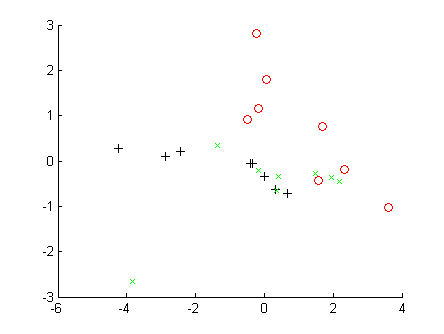
\includegraphics[width=80mm]{paclassplot.png}
\caption{Scatter plot shows dependency between first two principal components used and actual class of an object. Plus signs indicate "paper" sign , crosses indicate "rock" sign, circles indicate "scissors" sign. }
\label{fig:paclassplot}
\end{center}
\end{figure}

Cross validation test results showed that best accuracy over both test data and validation data was achieved by using combination of Hu moments and temporal area of the extracted object as features of the motion image and multi-class SVM for classification. Results for using different feature set are shown in Table \ref{tab:features}, for using different number of principal components are shown in Table \ref{tab:pca} and for using different classifiers in Table \ref{tab:classify}.

\begin{table}
\begin{center}
\begin{tabular}{| l | r | r |}
\hline
Features & Test set & Validation set \\ \hline
Temporal area of object only & & \\
Hu moments only & & \\
Both & & 87.5\% \\
\hline
\end{tabular}
\end{center}
\caption{Cross validation results when using different sets of feature.}
\label{tab:features}
\end{table}


\begin{table}
\begin{center}
\begin{tabular}{| l | r | r |}
\hline
Number of PC & Test set & Validation set \\ \hline
3 & & \% \\
4 & & \% \\
5 & & 87.5\% \\
6 & & \% \\
7 & & \% \\
\hline
\end{tabular}
\end{center}
\caption{Cross validation results when using different number of principal components.}
\label{tab:pca}
\end{table}

\begin{table}
\begin{center}
\begin{tabular}{| l | r | r |}
\hline
Number of PC & Test set & Validation set \\ \hline
RBF & &  \\
MLP & &  \\
Multi-class SVM & & 87.5\% \\
\hline
\end{tabular}
\end{center}
\caption{Cross validation results when using different classifiers.}
\label{tab:pca}
\end{table}